\documentclass[a4paper, 11pt]{article}
\usepackage[UTF8, scheme = plain]{ctex}
\usepackage{xcolor}     %高亮使用的颜色
\usepackage{amsmath}
\usepackage{graphicx}
\usepackage{geometry}
\usepackage{listings}
\geometry{scale=0.8}
\linespread{1.5}
\usepackage{hyperref}

\title{	
\normalfont \normalsize
\textsc{School of Data and Computer Science, Sun Yat-sen University} \\ [25pt] %textsc small capital letters
\rule{\textwidth}{0.5pt} \\[0.4cm] % Thin top horizontal rule
\huge  E03 Othello Game ($\alpha-\beta$ pruning) \\ % The assignment title
\rule{\textwidth}{2pt} \\[0.5cm] % Thick bottom horizontal rule
\author{20214810 Suixin Ou\and20214966 Yangkai Lin}
\date{\normalsize September 14, 2020} 
}

\begin{document}
\maketitle
\tableofcontents
\newpage

\section{Othello}
Othello (or Reversi) is a strategy board game for two players, played on an $8 \times 8$ uncheckered board. There are sixty-four identical game pieces called disks (often spelled "discs"), which are light on one side and dark on the other. Please see figure \ref{fig:othello}.

Players take turns placing disks on the board with their assigned color facing up. During a play, any disks of the opponent's color that are in a straight line and bounded by the disk just placed and another disk of the current player's color are turned over to the current player's color.

The object of the game is to have the majority of disks turned to display your color when the last playable empty square is filled.
\begin{figure}
  \centering
  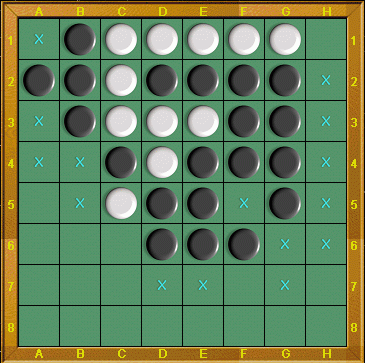
\includegraphics[width=6cm]{Pic/othello}
  \qquad
  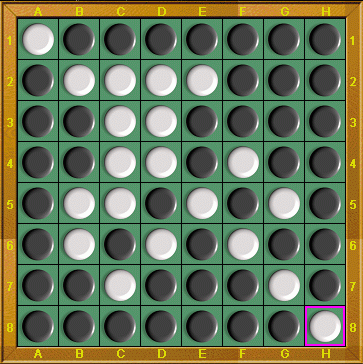
\includegraphics[width=6cm]{Pic/othello2}
  \caption{Othello Game}
  \label{fig:othello}
\end{figure}

You can refer to \url{http://www.tothello.com/html/guideline_of_reversed_othello.html} for more information of guideline, meanwhile, you can download the software to have a try from \url{http://www.tothello.com/html/download.html}. The game installer \texttt{tothello\_trial\_setup.exe} can also be found in the current folder.



\section{Tasks}
\begin{enumerate}

\item In order to reduce the complexity of the game, we think the board is $6\times 6$.

\item There are several evaluation functions that involve many aspects, you can turn to \url{http://www.cs.cornell.edu/~yuli/othello/othello.html} for help. In order to reduce the difficulty of the task, I have gaven you some hints of evaluation function in the file \texttt{Heuristic Function for Reversi (Othello).cpp}.

\item Please choose an appropriate evaluation function and use min-max and $\alpha-\beta$ prunning to implement the Othello game. The framework file you can refer to is \texttt{Othello.cpp}. Of course, I wish your program can beat the computer.

\item Write the related codes and take a screenshot of the running results in the file named \textsf{E03\_StudentNumber.pdf}, and send it to \textsf{ai\_2020@foxmail.com}, the \textbf{deadline} is 2020.09.20 23:59:59.
\end{enumerate}

\section{Codes}
\definecolor{mygreen}{rgb}{0,0.6,0}
\definecolor{mygray}{rgb}{0.5,0.5,0.5}
\definecolor{mymauve}{rgb}{0.58,0,0.82}
\lstset{
    backgroundcolor=\color{lightgray}, 
    basicstyle = \footnotesize,       
    breakatwhitespace = false,        
    breaklines = true,                 
    captionpos = b,                    
    commentstyle = \color{mygreen}\bfseries,
    extendedchars = false,             
    frame =shadowbox, 
    framerule=0.5pt,
    keepspaces=true,
    keywordstyle=\color{blue}\bfseries, % keyword style
    language = C++,                     % the language of code
    otherkeywords={string}, 
    numbers=left, 
    numbersep=5pt,
    numberstyle=\tiny\color{mygray},
    rulecolor=\color{black},         
    showspaces=false,  
    showstringspaces=false, 
    showtabs=false,    
    stepnumber=1,         
    stringstyle=\color{mymauve},        % string literal style
    tabsize=2,          
    title=\lstname                      
}
\begin{lstlisting}
#include <iostream>
#include <stdlib.h>

using namespace std;

int const MAX = 65534;

int  deepth = 10;         //最大搜索深度  (可调节)

int depth = 10;

//基本元素   棋子,颜色,数字变量

enum Option
{
    WHITE = -1, SPACE, BLACK	//是否能落子  //黑子
};

struct Do
{
    pair<int , int > pos;	
    int score;
};

struct WinNum
{	enum Option color;
    int stable;										// 此次落子赢棋个数
};							





//主要功能    棋盘及关于棋子的所有操作,功能
struct Othello														    
{

    WinNum cell[6][6];													//定义棋盘中有6*6个格子
    int whiteNum;														//白棋数目
    int blackNum;														//黑棋数


    void Create(Othello *board);										//初始化棋盘
    void Copy(Othello *boardDest, const  Othello *boardSource);			//复制棋盘
    void Show(Othello *board);											//显示棋盘
    int Rule(Othello *board, enum Option player);						//判断落子是否符合规则
    int Action(Othello *board, Do *choice, enum Option player);			//落子,并修改棋盘
    void Stable(Othello *board);										//计算赢棋个数
    int Judge(Othello *board, enum Option player);						//计算本次落子分数
    int Heuristic_Evaluation_Function(Othello *board, enum Option player); //计算本次落子分数
};//主要功能








//最大最小博弈与α-β剪枝 
Do * Find(Othello *board, enum Option player, int step, int min, int max, Do *choice)
{
    int i, j, k, num;
    Do *allChoices;
    choice->score = -MAX;
    choice->pos.first = -1;
    choice->pos.second = -1;

    num = board->Rule(board, player);
    if (num == 0)    /* 无处落子 */
    {
        if (board->Rule(board, (enum Option) - player))    /* 对方可以落子,让对方下.*/
        {
            Othello tempBoard;
            Do nextChoice;
            Do *pNextChoice = &nextChoice;
            board->Copy(&tempBoard, board);
            pNextChoice = Find(&tempBoard, (enum Option) - player, step - 1, -max, -min, pNextChoice);
            choice->score = -pNextChoice->score;
            choice->pos.first = -1;
            choice->pos.second = -1;
            return choice;
        }
        else    /* 对方也无处落子,游戏结束. */
        {
            int value = WHITE*(board->whiteNum) + BLACK*(board->blackNum);
            if (player*value>0)
            {
                choice->score = MAX - 1;
            }
            else if (player*value<0)
            {
                choice->score = -MAX + 1;
            }
            else
            {
                choice->score = 0;
            }
            return choice;
        }
    }
    if (step <= 0)    /* 已经考虑到step步,直接返回得分 */
    {
        choice->score = board->Judge(board, player);
        return choice;
    }

    allChoices = (Do *)malloc(sizeof(Do)*num);
    k = 0;
    for (i = 0; i<6; i++)
    {
        for (j = 0; j<6; j++)
        {
            if (i == 0 || i == 5 || j == 0 || j == 5)
            {
                if (board->cell[i][j].color == SPACE && board->cell[i][j].stable)
                {
                    allChoices[k].score = -MAX;
                    allChoices[k].pos.first = i;
                    allChoices[k].pos.second = j;
                    k++;
                }
            }
        }
    }

    for (i = 0; i<6; i++)
    {
        for (j = 0; j<6; j++)
        {
            if ((i == 2 || i == 3 || j == 2 || j == 3) && (i >= 2 && i <= 3 && j >= 2 && j <= 3))
            {
                if (board->cell[i][j].color == SPACE && board->cell[i][j].stable)
                {
                    allChoices[k].score = -MAX;
                    allChoices[k].pos.first = i;
                    allChoices[k].pos.second = j;
                    k++;
                }
            }
        }
    }

    for (i = 0; i<6; i++)
    {
        for (j = 0; j<6; j++)
        {
            if ((i == 1 || i == 4 || j == 1 || j == 4) && (i >= 1 && i <= 4 && j >= 1 && j <= 4))
            {
                if (board->cell[i][j].color == SPACE && board->cell[i][j].stable)
                {
                    allChoices[k].score = -MAX;
                    allChoices[k].pos.first = i;
                    allChoices[k].pos.second = j;
                    k++;
                }
            }
        }
    }

    for (k = 0; k<num; k++)
    {
        Othello tempBoard;
        Do thisChoice, nextChoice;
        Do *pNextChoice = &nextChoice;
        thisChoice = allChoices[k];
        board->Copy(&tempBoard, board);
        board->Action(&tempBoard, &thisChoice, player);
        pNextChoice = Find(&tempBoard, (enum Option) - player, step - 1, -max, -min, pNextChoice);
        thisChoice.score = -pNextChoice->score;

        if (thisChoice.score>min && thisChoice.score<max)    /* 可以预计的更优值 */
        {
            min = thisChoice.score;
            choice->score = thisChoice.score;
            choice->pos.first = thisChoice.pos.first;
            choice->pos.second = thisChoice.pos.second;
        }
        else if (thisChoice.score >= max)    /* 好的超乎预计 */
        {
            choice->score = thisChoice.score;
            choice->pos.first = thisChoice.pos.first;
            choice->pos.second = thisChoice.pos.second;
            break;
        }
        /* 不如已知最优值 */
    }
    free(allChoices);
    return choice;
}

Do * My_Find(Othello *board, enum Option player, int step, int min, int max, Do *choice)
{
    int i, j, k, num;
    Do *allChoices;
    choice->score = -MAX;
    choice->pos.first = -1;
    choice->pos.second = -1;

    num = board->Rule(board, player);
    if (num == 0)    /* 无处落子 */
    {
        if (board->Rule(board, (enum Option) - player))    /* 对方可以落子,让对方下.*/
        {
            Othello tempBoard;
            Do nextChoice;
            Do *pNextChoice = &nextChoice;
            board->Copy(&tempBoard, board);
            pNextChoice = My_Find(&tempBoard, (enum Option) - player, step - 1, -max, -min, pNextChoice);
            choice->score = -pNextChoice->score;
            choice->pos.first = -1;
            choice->pos.second = -1;
            return choice;
        }
        else    /* 对方也无处落子,游戏结束. */
        {
            int value = WHITE*(board->whiteNum) + BLACK*(board->blackNum);
            if (player*value>0)
            {
                choice->score = MAX - 1;
            }
            else if (player*value<0)
            {
                choice->score = -MAX + 1;
            }
            else
            {
                choice->score = 0;
            }
            return choice;
        }
    }
    if (step <= 0)    /* 已经考虑到step步,直接返回得分 */
    {
        choice->score = board->Heuristic_Evaluation_Function(board, player);
        return choice;
    }

    allChoices = (Do *)malloc(sizeof(Do)*num);
    k = 0;
    for (i = 0; i<6; i++)
    {
        for (j = 0; j<6; j++)
        {
            if (i == 0 || i == 5 || j == 0 || j == 5)
            {
                if (board->cell[i][j].color == SPACE && board->cell[i][j].stable)
                {
                    allChoices[k].score = -MAX;
                    allChoices[k].pos.first = i;
                    allChoices[k].pos.second = j;
                    k++;
                }
            }
        }
    }

    for (i = 0; i<6; i++)
    {
        for (j = 0; j<6; j++)
        {
            if ((i == 2 || i == 3 || j == 2 || j == 3) && (i >= 2 && i <= 3 && j >= 2 && j <= 3))
            {
                if (board->cell[i][j].color == SPACE && board->cell[i][j].stable)
                {
                    allChoices[k].score = -MAX;
                    allChoices[k].pos.first = i;
                    allChoices[k].pos.second = j;
                    k++;
                }
            }
        }
    }

    for (i = 0; i<6; i++)
    {
        for (j = 0; j<6; j++)
        {
            if ((i == 1 || i == 4 || j == 1 || j == 4) && (i >= 1 && i <= 4 && j >= 1 && j <= 4))
            {
                if (board->cell[i][j].color == SPACE && board->cell[i][j].stable)
                {
                    allChoices[k].score = -MAX;
                    allChoices[k].pos.first = i;
                    allChoices[k].pos.second = j;
                    k++;
                }
            }
        }
    }

    for (k = 0; k<num; k++)
    {
        Othello tempBoard;
        Do thisChoice, nextChoice;
        Do *pNextChoice = &nextChoice;
        thisChoice = allChoices[k];
        board->Copy(&tempBoard, board);
        board->Action(&tempBoard, &thisChoice, player);
        pNextChoice = My_Find(&tempBoard, (enum Option) - player, step - 1, -max, -min, pNextChoice);
        thisChoice.score = -pNextChoice->score;

        if (thisChoice.score>min && thisChoice.score<max)    /* 可以预计的更优值 */
        {
            min = thisChoice.score;
            choice->score = thisChoice.score;
            choice->pos.first = thisChoice.pos.first;
            choice->pos.second = thisChoice.pos.second;
        }
        else if (thisChoice.score >= max)    /* 好的超乎预计 */
        {
            choice->score = thisChoice.score;
            choice->pos.first = thisChoice.pos.first;
            choice->pos.second = thisChoice.pos.second;
            break;
        }
        /* 不如已知最优值 */
    }
    free(allChoices);
    return choice;
}

int main()					
{
    Othello board;
    Othello *pBoard = &board;
    enum Option player , present ;
    Do choice;
    Do *pChoice = &choice;
    int  num , result = 0;
    char restart = ' ';

start:						
    player = SPACE;			
    present = BLACK;                  
    num = 4;
    restart = ' ';
    
    cout << ">>>人机对战开始: \n";
    
    
        

        while (player != WHITE && player != BLACK)
        {
            cout << ">>>请选择执黑棋(○),或执白棋(●):输入1为黑棋,-1为白棋" << endl;
            scanf("%d", &player);
            cout << ">>>黑棋行动:  \n";

            
            if (player != WHITE && player != BLACK)
            {
                cout << "输入不符合规范,请重新输入\n";
            }
        }

        board.Create(pBoard);					

        while (num<36)													// 棋盘上未下满36子 
        {
            char *Player = "";
            if (present == BLACK)
            {
                Player = "黑棋(○)";
            }
            else if (present == WHITE)
            {
                Player = "白棋(●)";
            }

            if (board.Rule(pBoard, present) == 0)						//未下满并且无子可下
            {
                if (board.Rule(pBoard, (enum Option) - present) == 0)
                {
                    break;                 
                }

                cout << Player << "GAME OVER! \n";
            }
            else
            {
                int i, j;
                //board.Show(pBoard);

                if (present == player)     
                {
                    /*
                    while (1)
                    {
                        cout << Player << " \n >>>请输入棋子坐标(空格相隔 如“3 5”代表第3行第5列):\n";
                        
                        cin >> i>> j;		
                        i--;
                        j--;
                        pChoice->pos.first = i;
                        pChoice->pos.second = j;

                        if (i<0 || i>5 || j<0 || j>5 || pBoard->cell[i][j].color != SPACE || pBoard->cell[i][j].stable == 0)
                        {
                            cout <<">>>此处落子不符合规则,请重新选择   \n";
                            board.Show(pBoard);
                        }
                        else
                        {
                            break;
                        }
                    }
                    system("cls");
                    cout << ">>>玩家 本手棋得分为     " << pChoice->score << endl;
                    system("pause");
                    cout << ">>>按任意键继续" << pChoice->score << endl;
                    */
                    //cout << Player << "..........................";
                    
                    pChoice = My_Find(pBoard, present, depth, -MAX, MAX, pChoice);
                    i = pChoice->pos.first;
                    j = pChoice->pos.second;
                    //system("cls");
                }
                else   //AI下棋
                {   
                    //cout << Player << "..........................";
                    
                    pChoice = Find(pBoard, present, deepth, -MAX, MAX, pChoice);
                    i = pChoice->pos.first;
                    j = pChoice->pos.second;
                    //system("cls");
                    //cout << ">>>AI 本手棋得分为     " << pChoice->score << endl;
                }


                board.Action(pBoard, pChoice, present);
                num++;
                //cout << Player << ">>>AI于" << i + 1 << "," << j + 1<<"落子";
                cout << Player << "于" << i + 1 << "," << j + 1<<"落子。黑棋数:"<<pBoard->blackNum<<",白棋数:"<<pBoard->whiteNum<<endl;
            }

            present = (enum Option) - present;    //交换执棋者
        }


        //board.Show(pBoard);


        result = pBoard->whiteNum - pBoard->blackNum;

        if (result>0)
        {
            cout << "\n——————白棋(●)胜——————\n";
        }
        else if (result<0)
        {
            cout << "\n——————黑棋(○)胜——————\n";
        }
        else
        {
            cout << "\n————————平局————————\n";
        }

        cout << "\n ————————GAME OVER!————————\n";
        cout << "\n";
        
        while (restart != 'Y' && restart != 'N')
        {
            cout <<"|—————————————————————|\n";
            cout <<"|                                          | \n";
            cout <<"|                                          |   \n";
            cout <<"|>>>>>>>>>>>>>>>>Again?(Y,N)<<<<<<<<<<<<<<<|\n";
            cout <<"|                                          | \n";
            cout <<"|                                          |  \n";
            cout <<"|—————————————————————|\n";
            cout << "                                            \n";
            cout << "                                            \n";
            cout << "                                            \n";
            cout << " —————                 —————       \n";
            cout << " |   YES  |                 |   NO   |      \n";
            cout << " —————                 —————      \n";

            cin >> restart;
            if (restart == 'Y')
            {
                goto start;
            }
        }

    
    return 0;
}






void Othello::Create(Othello *board)
{
    int i, j;
    board->whiteNum = 2;
    board->blackNum = 2;
    for (i = 0; i<6; i++)
    {
        for (j = 0; j<6; j++)
        {
            board->cell[i][j].color = SPACE;
            board->cell[i][j].stable = 0;
        }
    }
    board->cell[2][2].color = board->cell[3][3].color = WHITE;
    board->cell[2][3].color = board->cell[3][2].color = BLACK;
}


void Othello::Copy(Othello *Fake, const  Othello *Source)
{
    int i, j;
    Fake->whiteNum = Source->whiteNum;
    Fake->blackNum = Source->blackNum;
    for (i = 0; i<6; i++)
    {
        for (j = 0; j<6; j++)
        {
            Fake->cell[i][j].color = Source->cell[i][j].color;
            Fake->cell[i][j].stable = Source->cell[i][j].stable;
        }
    }
}

void Othello::Show(Othello *board)
{
    int i, j;
    cout << "\n  ";
    for (i = 0; i<6; i++)
    {
        cout << "   " << i + 1;
    }
    cout << "\n    ────────────\n";
    for (i = 0; i<6; i++)
    {
        cout << i + 1 << "--│";
        for (j = 0; j<6; j++)
        {
            switch (board->cell[i][j].color)
            {
            case BLACK:
                cout << "○│";
                break;
            case WHITE:
                cout << "●│";
                break;
            case SPACE:
                if (board->cell[i][j].stable)
                {
                    cout << " +│";
                }
                else
                {
                    cout << "  │";
                }
                break;
            default:    /* 棋子颜色错误 */
                cout << "* │";
            }
        }
        cout << "\n    ────────────\n";
    }

    cout << ">>>白棋(●)个数为:" << board->whiteNum << "         ";
    cout << ">>>黑棋(○)个数为:" << board->blackNum << endl << endl << endl;
}


int Othello::Rule(Othello *board, enum Option player)
{
    int i, j;
    unsigned num = 0;
    for (i = 0; i<6; i++)
    {
        for (j = 0; j<6; j++)
        {
            if (board->cell[i][j].color == SPACE)
            {
                int x, y;
                board->cell[i][j].stable = 0;
                for (x = -1; x <= 1; x++)
                {
                    for (y = -1; y <= 1; y++)
                    {
                        if (x || y)    /* 8个方向 */
                        {
                            int i2, j2;
                            unsigned num2 = 0;
                            for (i2 = i + x, j2 = j + y; i2 >= 0 && i2 <= 5 && j2 >= 0 && j2 <= 5; i2 += x, j2 += y)
                            {
                                if (board->cell[i2][j2].color == (enum Option) - player)
                                {
                                    num2++;
                                }
                                else if (board->cell[i2][j2].color == player)
                                {
                                    board->cell[i][j].stable += player*num2;
                                    break;
                                }
                                else if (board->cell[i2][j2].color == SPACE)
                                {
                                    break;
                                }
                            }
                        }
                    }
                }

                if (board->cell[i][j].stable)
                {
                    num++;
                }
            }
        }
    }
    return num;
}


int Othello::Action(Othello *board, Do *choice, enum Option player)
{
    int i = choice->pos.first, j = choice->pos.second;
    int x, y;

    if (board->cell[i][j].color != SPACE || board->cell[i][j].stable == 0 || player == SPACE)
    {
        return -1;
    }


    board->cell[i][j].color = player;
    board->cell[i][j].stable = 0;


    if (player == WHITE)
    {
        board->whiteNum++;
    }
    else if (player == BLACK)
    {
        board->blackNum++;
    }



    for (x = -1; x <= 1; x++)
    {
        for (y = -1; y <= 1; y++)
        {

            //需要在每个方向(8个)上检测落子是否符合规则(能否吃子)


            if (x || y)
            {
                int i2, j2;
                unsigned num = 0;
                for (i2 = i + x, j2 = j + y; i2 >= 0 && i2 <= 5 && j2 >= 0 && j2 <= 5; i2 += x, j2 += y)
                {
                    if (board->cell[i2][j2].color == (enum Option) - player)
                    {
                        num++;
                    }
                    else if (board->cell[i2][j2].color == player)
                    {
                        board->whiteNum += (player*WHITE)*num;
                        board->blackNum += (player*BLACK)*num;

                        for (i2 -= x, j2 -= y; num>0; num--, i2 -= x, j2 -= y)
                        {
                            board->cell[i2][j2].color = player;
                            board->cell[i2][j2].stable = 0;
                        }
                        break;
                    }
                    else if (board->cell[i2][j2].color == SPACE)
                    {
                        break;
                    }
                }
            }
        }
    }
    return 0;
}


void Othello::Stable(Othello *board)
{
    int i, j;
    for (i = 0; i<6; i++)
    {
        for (j = 0; j<6; j++)
        {
            if (board->cell[i][j].color != SPACE)
            {
                int x, y;
                board->cell[i][j].stable = 1;

                for (x = -1; x <= 1; x++)
                {
                    for (y = -1; y <= 1; y++)
                    {
                        /* 4个方向 */
                        if (x == 0 && y == 0)
                        {
                            x = 2;
                            y = 2;
                        }
                        else
                        {
                            int i2, j2, flag = 2;
                            for (i2 = i + x, j2 = j + y; i2 >= 0 && i2 <= 5 && j2 >= 0 && j2 <= 5; i2 += x, j2 += y)
                            {
                                if (board->cell[i2][j2].color != board->cell[i][j].color)
                                {
                                    flag--;
                                    break;
                                }
                            }

                            for (i2 = i - x, j2 = j - y; i2 >= 0 && i2 <= 5 && j2 >= 0 && j2 <= 5; i2 -= x, j2 -= y)
                            {
                                if (board->cell[i2][j2].color != board->cell[i][j].color)
                                {
                                    flag--;
                                    break;
                                }
                            }

                            if (flag)    /* 在某一条线上稳定 */
                            {
                                board->cell[i][j].stable++;
                            }
                        }
                    }
                }
            }
        }
    }
}

int Othello::Judge(Othello *board, enum Option player)
{
    int value = 0;
    int i, j;
    Stable(board);
    for (i = 0; i<6; i++)
    {
        for (j = 0; j<6; j++)
        {
            value += (board->cell[i][j].color)*(board->cell[i][j].stable);
        }
    }

    value += 64 * board->cell[0][0].color;
    value += 64 * board->cell[0][5].color;
    value += 64 * board->cell[5][0].color;
    value += 64 * board->cell[5][5].color;
    value -= 32 * board->cell[1][1].color;
    value -= 32 * board->cell[1][4].color;
    value -= 32 * board->cell[4][1].color;
    value -= 32 * board->cell[4][4].color;

    return value*player;
}

bool canmove(Option self, Option opp, Option* str) {
    if (str[0] != opp) return false;
    for (int ctr = 1; ctr < 8; ctr++) {
        if (str[ctr] == SPACE) return false;
        if (str[ctr] == self) return true;
    }
    return false;
}

bool isLegalMove(Option self, Option opp, Othello *board, int startx, int starty) {
    if (board->cell[startx][starty].color != SPACE) return false;
    Option str[10];
    int x, y, dx, dy, ctr;
    for (dy = -1; dy <= 1; dy++)
        for (dx = -1; dx <= 1; dx++) {
            // keep going if both velocities are zero
            if (!dy && !dx) continue;
            str[0] = SPACE;
            for (ctr = 1; ctr < 8; ctr++) {
                x = startx + ctr * dx;
                y = starty + ctr * dy;
                if (x >= 0 && y >= 0 && x < 8 && y < 8) str[ctr - 1] = board->cell[x][y].color;
                else str[ctr - 1] = SPACE;
            }
            if (canmove(self, opp, str)) return true;
        }
    return false;
}

int num_valid_moves(Option self, Option opp, Othello *board) {
    int count = 0, i, j;
    for (i = 0; i < 8; i++)
        for (j = 0; j < 8; j++)
            if (isLegalMove(self, opp, board, i, j)) count++;
    return count;
}

int Othello::Heuristic_Evaluation_Function(Othello *board, enum Option player)
{
    /*
    int value = 0;
    int i, j;
    for (i = 0; i<6; i++)
    {
        for (j = 0; j<6; j++)
        {
            value += board->cell[i][j].color == player;
        }
    }

    value += 100 * board->Rule(board, player);

    value += 1000 * (board->cell[0][0].color == player);
    value += 1000 * (board->cell[0][5].color == player);
    value += 1000 * (board->cell[5][0].color == player);
    value += 1000 * (board->cell[5][5].color == player);

    return value;
    */
    int my_tiles = 0, opp_tiles = 0, i, j, k, my_front_tiles = 0, opp_front_tiles = 0, x, y;
    double p = 0, c = 0, l = 0, m = 0, f = 0, d = 0;

    int X1[] = {-1, -1, 0, 1, 1, 1, 0, -1};
    int Y1[] = {0, 1, 1, 1, 0, -1, -1, -1};
    int V[6][6] = {{20, -3, 8, 8, -3, 20},
                   {-3, -7, 1, 1, -7, -3},
                   {8, 1, -3, -3, 1, 8},
                   {8, 1, -3, -3, 1, 8},
                   {-3, -7, 1, 1, -7, -3},
                   {20, -3, 8, 8, -3, 20}};

    // Piece difference, frontier disks and disk squares
    for(i=0; i<6; i++)
        for(j=0; j<6; j++)  {
            if(board->cell[i][j].color == player)  {
                d += V[i][j];
                my_tiles++;
            } else if(board->cell[i][j].color == (enum Option)-player)  {
                d -= V[i][j];
                opp_tiles++;
            }
            if(board->cell[i][j].color != SPACE)   {
                for(k=0; k<8; k++)  {
                    x = i + X1[k]; y = j + Y1[k];
                    if(x >= 0 && x < 6 && y >= 0 && y < 6 && board->cell[x][y].color == SPACE) {
                        if(board->cell[i][j].color == player)  my_front_tiles++;
                        else opp_front_tiles++;
                        break;
                    }
                }
            }
        }
    if(my_tiles > opp_tiles)
        p = (100.0 * my_tiles)/(my_tiles + opp_tiles);
    else if(my_tiles < opp_tiles)
        p = -(100.0 * opp_tiles)/(my_tiles + opp_tiles);
    else p = 0;

    if(my_front_tiles > opp_front_tiles)
        f = -(100.0 * my_front_tiles)/(my_front_tiles + opp_front_tiles);
    else if(my_front_tiles < opp_front_tiles)
        f = (100.0 * opp_front_tiles)/(my_front_tiles + opp_front_tiles);
    else f = 0;

// Corner occupancy
    my_tiles = opp_tiles = 0;
    if(board->cell[0][0].color == player) my_tiles++;
    else if(board->cell[0][0].color == (enum Option)-player) opp_tiles++;
    if(board->cell[0][5].color == player) my_tiles++;
    else if(board->cell[0][5].color == (enum Option)-player) opp_tiles++;
    if(board->cell[5][0].color == player) my_tiles++;
    else if(board->cell[5][0].color == (enum Option)-player) opp_tiles++;
    if(board->cell[5][5].color == player) my_tiles++;
    else if(board->cell[5][5].color == (enum Option)-player) opp_tiles++;
    c = 25 * (my_tiles - opp_tiles);

    // Corner occupancy
    my_tiles = opp_tiles = 0;
    if (board->cell[0][0].color == player) my_tiles++;
    else if (board->cell[0][0].color == (enum Option) - player) opp_tiles++;
    if (board->cell[0][5].color == player) my_tiles++;
    else if (board->cell[0][5].color == (enum Option) - player) opp_tiles++;
    if (board->cell[5][0].color == player) my_tiles++;
    else if (board->cell[5][0].color == (enum Option) - player) opp_tiles++;
    if (board->cell[5][5].color == player) my_tiles++;
    else if (board->cell[5][5].color == (enum Option) - player) opp_tiles++;
    c = 25 * (my_tiles - opp_tiles);

    // Corner closeness
    my_tiles = opp_tiles = 0;
    if (board->cell[0][0].color != SPACE) {
        if (board->cell[0][1].color == player) my_tiles++;
        else if (board->cell[0][1].color == (enum Option) - player) opp_tiles++;
        if (board->cell[1][1].color == player) my_tiles++;
        else if (board->cell[1][1].color == (enum Option) - player) opp_tiles++;
        if (board->cell[1][0].color == player) my_tiles++;
        else if (board->cell[1][0].color == (enum Option) - player) opp_tiles++;
    }
    if (board->cell[0][5].color != SPACE) {
        if (board->cell[0][4].color == player) my_tiles++;
        else if (board->cell[0][4].color == (enum Option) - player) opp_tiles++;
        if (board->cell[1][5].color == player) my_tiles++;
        else if (board->cell[1][5].color == (enum Option) - player) opp_tiles++;
        if (board->cell[1][4].color == player) my_tiles++;
        else if (board->cell[1][4].color == (enum Option) - player) opp_tiles++;
    }
    if (board->cell[5][0].color != SPACE) {
        if (board->cell[5][1].color == player) my_tiles++;
        else if (board->cell[5][1].color == (enum Option) - player) opp_tiles++;
        if (board->cell[1][5].color == player) my_tiles++;
        else if (board->cell[4][1].color == (enum Option) - player) opp_tiles++;
        if (board->cell[1][4].color == player) my_tiles++;
        else if (board->cell[4][0].color == (enum Option) - player) opp_tiles++;
    }
    if (board->cell[5][5].color != SPACE) {
        if (board->cell[4][5].color == player) my_tiles++;
        else if (board->cell[4][5].color == (enum Option) - player) opp_tiles++;
        if (board->cell[4][4].color == player) my_tiles++;
        else if (board->cell[4][4].color == (enum Option) - player) opp_tiles++;
        if (board->cell[5][4].color == player) my_tiles++;
        else if (board->cell[5][4].color == (enum Option) - player) opp_tiles++;
    }
    l = -12.5 * (my_tiles - opp_tiles);

// Mobility
    my_tiles = num_valid_moves(player, (enum Option)-player, board);
    opp_tiles = num_valid_moves((enum Option)-player, player, board);
    if(my_tiles > opp_tiles)
        m = (100.0 * my_tiles)/(my_tiles + opp_tiles);
    else if(my_tiles < opp_tiles)
        m = -(100.0 * opp_tiles)/(my_tiles + opp_tiles);
    else m = 0;

// final weighted score
    double score = (10 * p) + (801.724 * c) + (38.2026 * l) + (78.922 * m) + (74.396 * f) + (10 * d);
    return (int)score;
}
\end{lstlisting}


\section{Results}
\begin{figure}[ht]
	\centering
	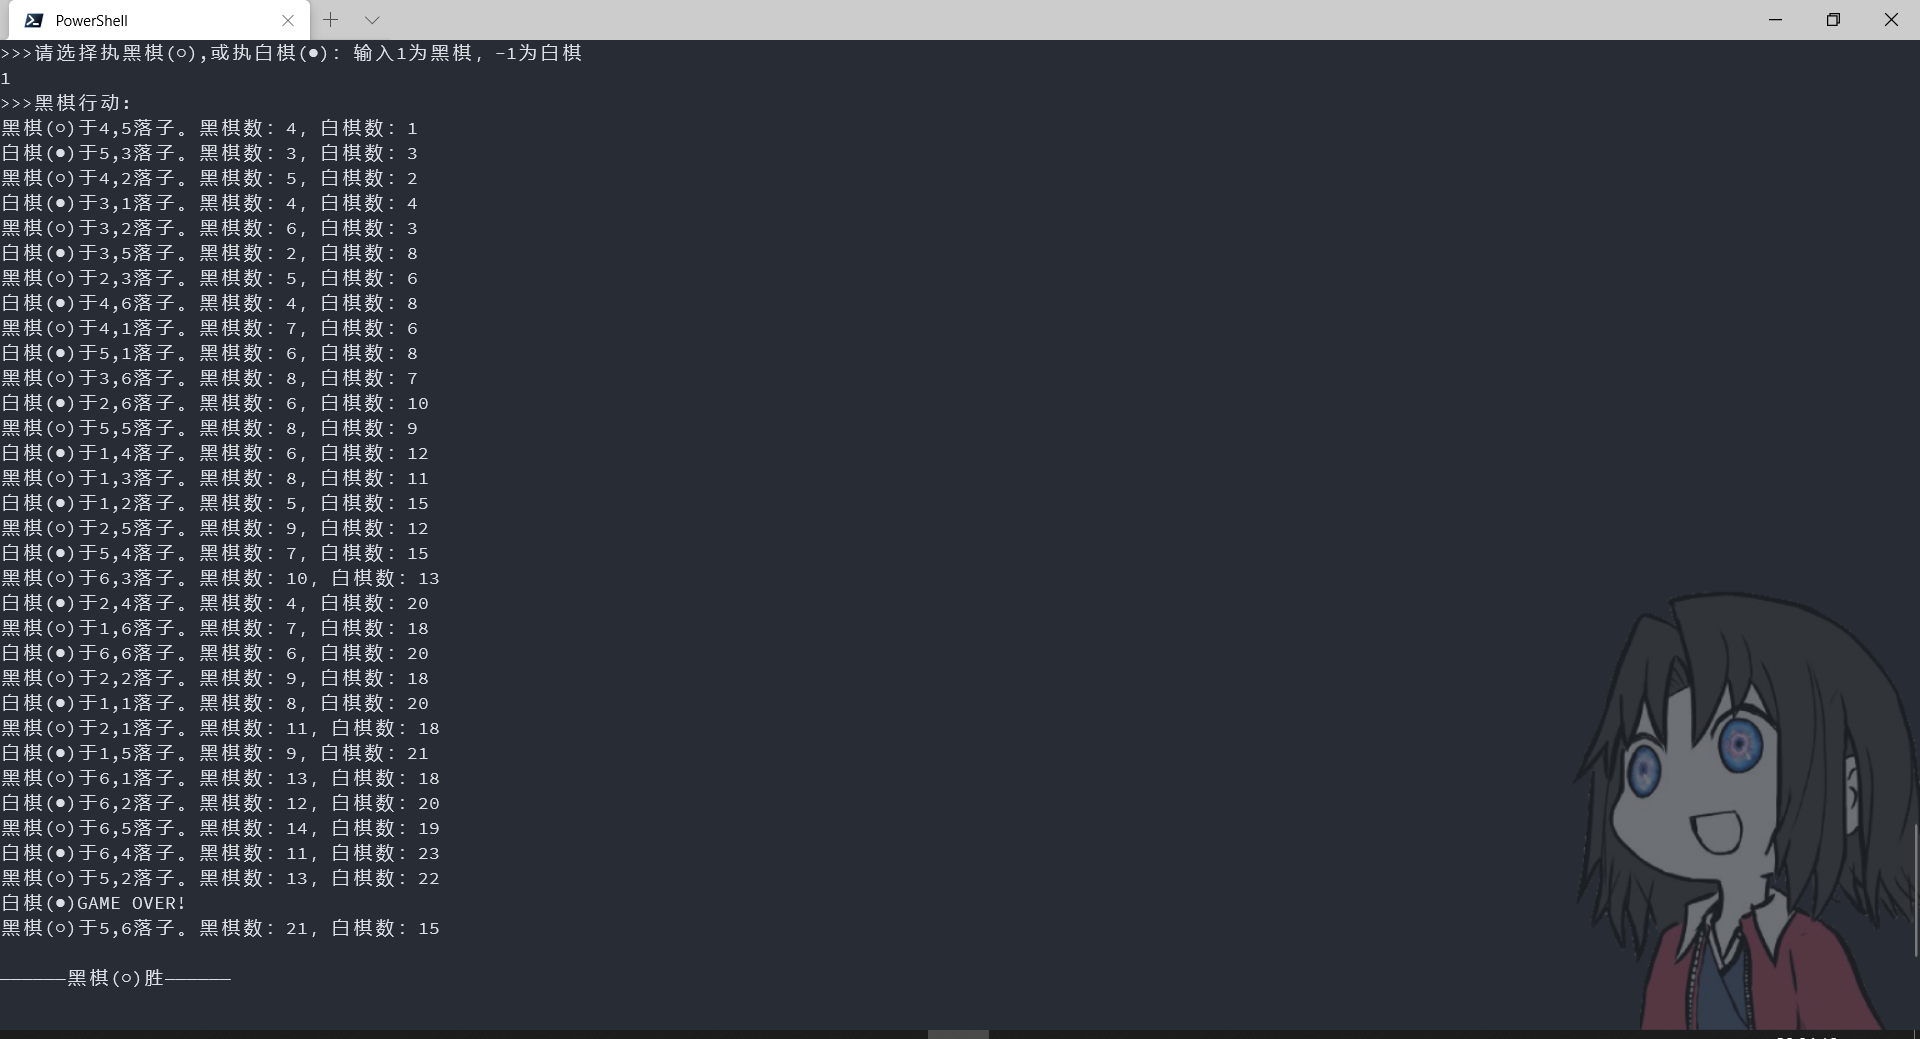
\includegraphics[width=15cm]{result1.png}
	\caption{result1}
	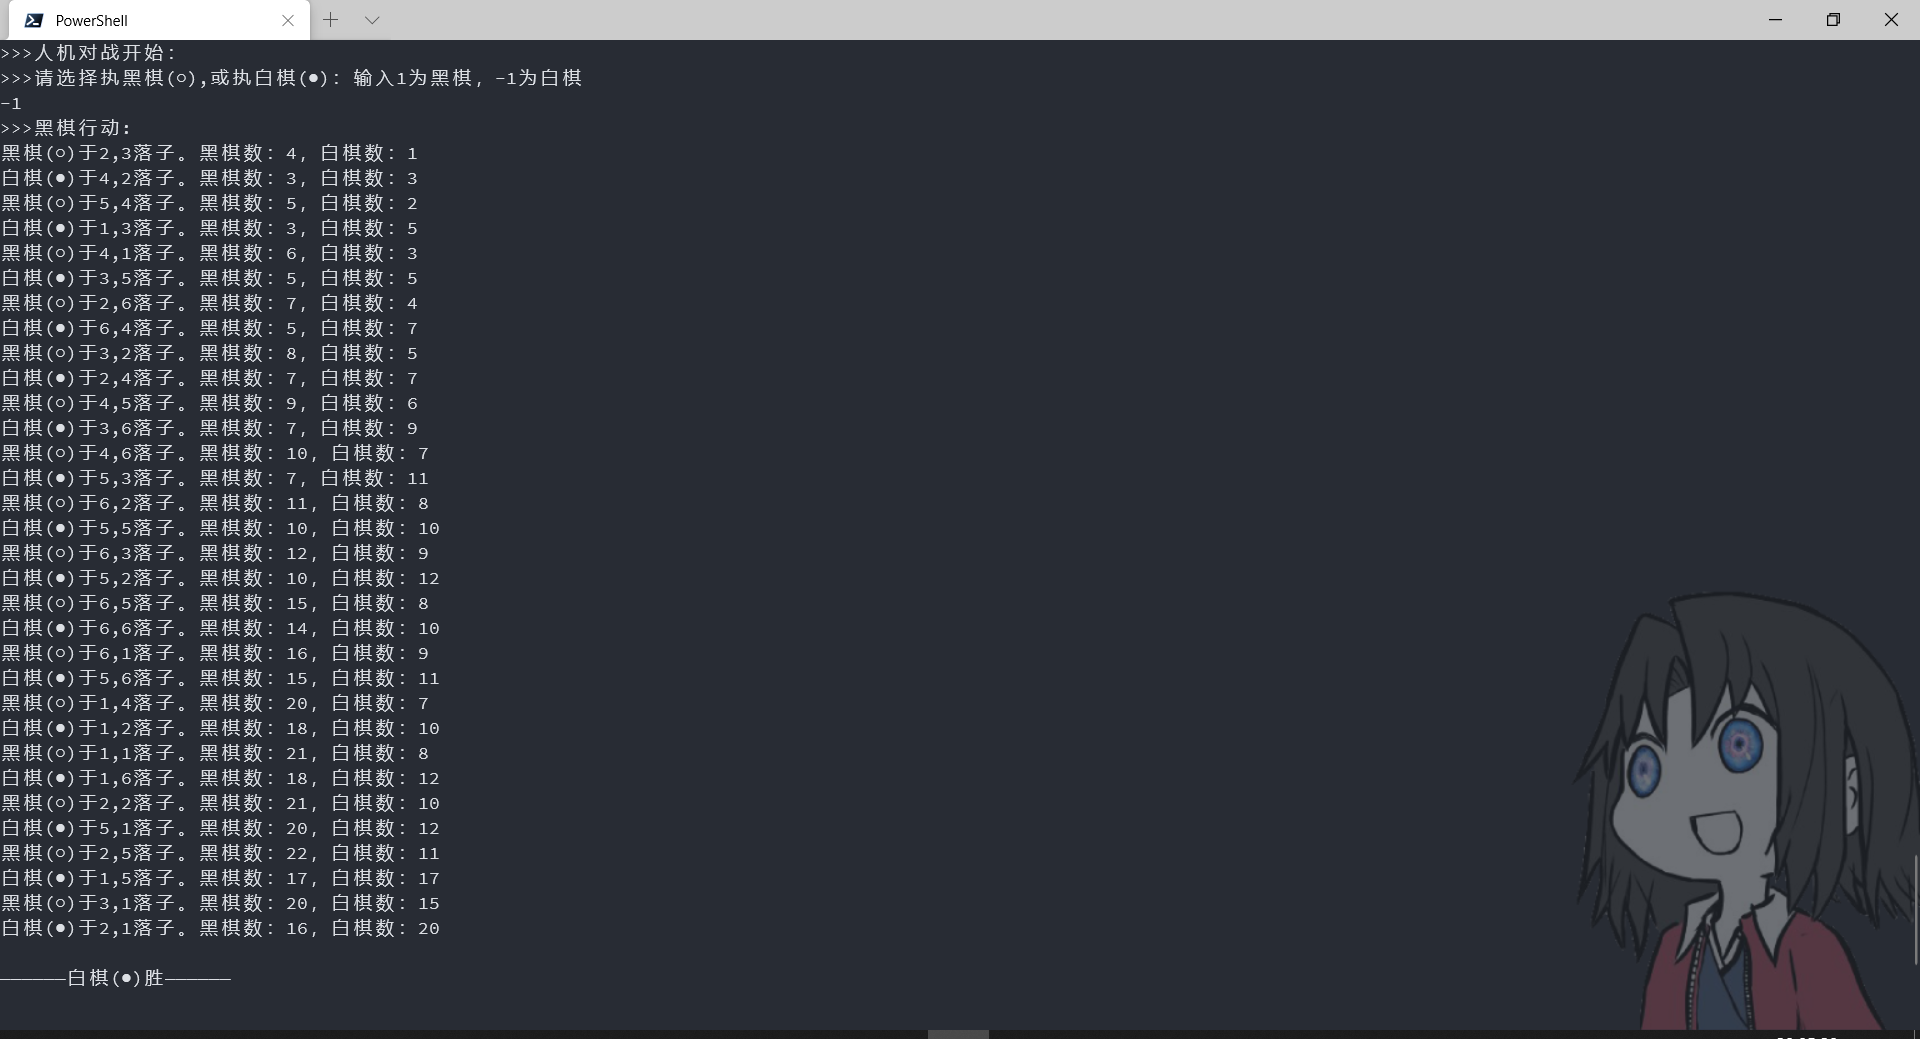
\includegraphics[width=15cm]{result2.png}
	\caption{result2}
\end{figure}


%\clearpage
%\bibliography{E:/Papers/LiuLab}
%\bibliographystyle{apalike}
\end{document} 
%%% Local Variables:
%%% mode: latex
%%% TeX-master: t
%%% End: